%!TEX program = xelatex
\def\footer#1{\def\insertfooter{#1}}
\documentclass[final]{beamer}
\usepackage[utf8]{inputenc}

\usepackage[scale=1.150]{beamerposter}
\usetheme{MUWposter} 

\usepackage{multicol}
\usepackage{array}
\usepackage{amsmath,bm,bbm}  
\usepackage{enumitem}
\usepackage{bbding}
\usepackage[portuguese,activeacute]{babel}
\usepackage{babelbib}
\newcolumntype{L}{>{\arraybackslash}m{22cm}}
\newcolumntype{S}{>{\arraybackslash}m{5cm}}
\usepackage{pgf}  
\usepackage{mathtools}
\usepackage{amsmath, amsthm, amssymb, amsfonts}
\usepackage{exscale}
\usepackage{xcolor}
\usepackage{ushort}
\usepackage{setspace}
\usepackage[square,numbers]{natbib}
\usepackage{url}
\bibliographystyle{abbrvnat}
\renewcommand{\vec}[1]{\ushort{#1}}
\renewcommand{\vec}[1]{\mathbf{#1}}
\definecolor{greenMUW}{RGB}{60,191,174}
\definecolor{blueMUW}{RGB}{17,29,79}
\definecolor{skinMUW}{RGB}{254,228,217}
\definecolor{hellblauMUW}{RGB}{95,180,229}
\usepackage{xcolor}
\usepackage{graphicx}
\colorlet{themecolor}{greenMUW}
\usebackgroundtemplate{
\includegraphics[width=80cm,height=120cm]{MUW_green}}


\setlength{\paperwidth}{80cm} 
\setlength{\paperheight}{120cm}
\newlength{\sepmargin}
\newlength{\sepwid}
\newlength{\onecolwid}
\newlength{\twocolwid}
\newlength{\threecolwid}

\setlength{\sepmargin}{0.055\paperwidth} 
\setlength{\sepwid}{0.03\paperwidth} 
\setlength{\onecolwid}{0.425\paperwidth} 
\setbeamertemplate{title}[left]
\setbeamertemplate{frametitle}[default][left]
%\setmainfont{Georgia}

\title{Análise de Sinais com Distâncias Estocásticas e Diferenças de Entropias - Ferramentas para Análise de Séries Temporais}

\author{Eduarda T.\ C.\ Chagas$^{1}$, Alejandro C.\ Frery$^{2}$} 

\institute{$^{1}$Estudante de IC de Ciência da Computação, Ufal\\
$^{2}$Pesquisador do LaCCAN, Ufal}

\usepackage[absolute,overlay]{textpos}
  \setlength{\TPHorizModule}{1mm}
  \setlength{\TPVertModule}{1mm}
  
\begin{document}

\begin{textblock}{500}(185,70)
\Large{1.03.02 - Ciência da Computação / Matemática da Computação}
\end{textblock}

\begin{textblock}{20}(650,190)

\includegraphics[width=10cm]{sbpc}
\end{textblock}

\begin{textblock}{20}(500,180)

\includegraphics[width=13cm]{laccan}
\end{textblock}

\addtobeamertemplate{block end}{}{\vspace*{1ex}}
\addtobeamertemplate{block alerted end}{}{\vspace*{0ex}} 
\setlength{\belowcaptionskip}{2ex} 
\setlength\belowdisplayshortskip{1ex}
  

\begin{frame}[t] 
\begin{columns}[t] 
\begin{column}{\onecolwid} 

\begin{block}{Introdução}
%\footnotesize
\small

\quad Séries temporais são conjunto de dados obtidos a partir de um processo observacional ao longo de um determinado período de tempo, não necessariamente dividido em espaços iguais, sendo caracterizadas pela dependência serial existente entre as observações.\newline

O projeto aqui relatado tomou como ponto de partida a identificação das necessidades dos pesquisadores: uma ferramenta gráfica amigável e funcionalidades rápidas, eficientes e numericamente confiáveis para a aplicação de técnicas não paramétricas à análise de séries temporais.
Outro requisito foi o da portabilidade para diversos sistemas operacionais e arquiteturas de hardware, e o uso de ferramentas FLOSS (\textit{Free/Libre Open Source Software}).\newline
 
Apresentamos, assim, o desenvolvimento de uma ferramenta portável, rápida e de boa qualidade numérica que possibilita análises interativas e exploratórias dos dados de uma série temporal através de técnicas provenientes da Teoria da Informação.
Com ela, o usuário dispõe de uma conjunto técnicas de análise presentes na literatura para processar e examinar seus dados de modo eficiente e com um mínimo período de aprendizado.
A ferramenta é extensível.\newline

\textbf{Palavras-chave:} Teoria da Informação, plataforma \texttt R, Estatística Computacional.\newline

\textbf{Apoio financeiro:} CNPq (Conselho Nacional de Desenvolvimento Científico e Tecnológico).
\end{block}
          
\begin{block}{Metodologia}
%\footnotesize
\small

\quad A primeira parte do projeto consistiu da apropriação do referencial teórico.
Seja a série temporal $\bm x = (x_1, x_2, \dots, x_n)$.
Ao invés de analisarmos os valores, transformaremos grupos de $N$ valores (não necessariamente adjacentes) e padrões ordinais, e analisaremos a sua distribuição de frequência.
Por exemplo e sem perda de generalidade, com $N=3$ e para qualquer $i$ viável,
se $x_i<x_{i+1}<x_{i+2}$ assignaremos a esta tripla o padrão $\pi_0$;
caso $x_i>x_{i+1}>x_{i+2}$ o padrão será $\pi_1$ e assim por diante.
Com isso, há $N!$ possíveis padrões.
Esta é conhecida como \textit{simbolização de Bandt \& Pompe}~\cite{PermutationEntropyBandtPompe}.\newline

Forma-se, então, um histograma e, a partir dele, extraem-se quantificadores como, por exemplo, entropia, distância estocástica a uma distribuição de equilíbrio, e complexidade estatística.\newline

Seja, assim, $\bm h=(h_1,\dots,h_{N!})$ o histograma de proporções dos $N!$ padrões observados a partir da série temporal $\bm x$.
Calculamos a entropia de Shannon

\begin{equation}
H(\bm h) = \sum_{i=1}^{N!} (-\log h_i) h_i,
\label{eq:Entropia}
\end{equation}

A entropia de Shannon é o primeiro elemento a descrever a nossa série temporal.
Ela mede a desordem do sistema que deu origem aos dados $\bm x$.\newline

Calculamos logo a distância de Jensen-Shannoon à distribuição uniforme $\bm u=(1/N!,\dots,1/N!)$
\begin{equation}
D(\bm h,\bm u) = \sum_{i=1}^{N!} \Big(h_i \log\frac{h_i}{u_i} +
u_i \log\frac{u_i}{p_i}
\Big),
\end{equation}

em que $u_i=1/N!$
Esta é uma medida de quão perto ou longe a dinâmica subjacente está de um processo sem informação nenhuma.\\

Finalmente, calculamos o terceiro descritor da nossa série temporal: a sua Complexidade Estatística:

\begin{equation}
C(\bm h, \bm u) = H(\bm h) D(\bm h, \bm u).
\end{equation}

Cada série temporal pode então ser descrita por um ponto $(H(\bm h), C(\bm h, \bm u))$.
O conjunto de todos os pares $(H(\bm h), C(\bm h, \bm u))$ para qualquer série temporal descrita por padrões de comprimento $N$ jaz em um subconjunto compacto $\mathbbm R^2$: o plano Entropia-Complexidade.\\

Embora aqui relatemos apenas o uso da entropia de Shannon e da distância de Jensen-Shannon, o sistema oferece outras entropias~\cite{salicruetal1993} e distâncias estocásticas~\cite{StatisticalInferenceBasedonDivergenceMeasures}.
\end{block} 
\end{column} 

\begin{column}{\onecolwid} 

\begin{block}{Resultados e discussões}
%\footnotesize
\small

\quad Seguindo o modelo de engenharia de software em espiral, o sistema foi projetado e desenvolvido de forma modular, composto pelas seguintes unidades:

\begin{itemize}[leftmargin=1.0in]
\item Módulo de simbolização;
\item Módulo de análise;
\item Modulo de visualização e interação (em fase de desenvolvimento);
\end{itemize}

Esses módulos foram e estão sendo desenvolvidos seguindo um cronograma. Depois passaram pelas seguintes etapas:

\begin{itemize}[leftmargin=1.0in]
\item Integração dos módulos em um sistema;
\item Teste e validação do sistema (em fase de desenvolvimento);
\item Geração da interface gráfica (em fase de desenvolvimento).
\end{itemize}

Permite-se a leitura de dados em vários formatos (TXT, CSV ou XLSX), e o usuário a seguir poderá escolher:

\begin{itemize}[leftmargin=1.0in]
	\item[\HandRight] Gerar o gráfico da série;
	\item[\HandRight] Calcular seus diversos valores de Entropia;
	\item[\HandRight] Calcular seus diversos valores de Distâncias estocásticas;
	\item[\HandRight] Calcular complexidades estatísticas;
    \item[\HandRight] Identificar padrões no gráfico da série temporal;
    \item[\HandRight] Gerar planos de Entropias;
    \item[\HandRight] Gerar planos de Distâncias estocásticas;
	\item[\HandRight] Gerar o histograma de padrões;
	\item[\HandRight] Identificar o ponto característico da série no plano Entropia-Complexidade.
\end{itemize}

Um elemento original do sistema é a vinculação entre o histograma de padrões e a série temporal. Escolhendo um ou mais elementos do histograma, os valores correspondentes na série temporal aparecem realçados.

\begin{center}\vspace{1cm}
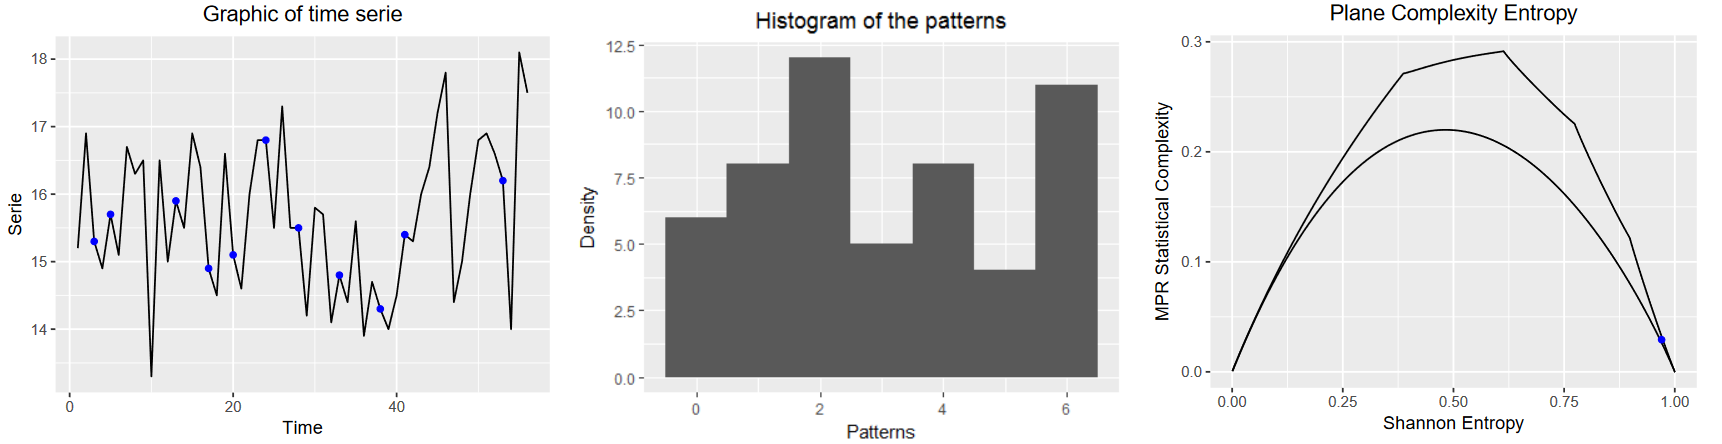
\includegraphics[width=1\linewidth]{img1}
\vspace*{1cm}
\textit{\footnotesize A figura acima ilustra o processo de extração de informações de uma série temporal. A imagem 1.1 nos informa a presença dos padrões $(2,1,3)$ na série. Já a imagem 1.2 apresenta o histograma de densidade, utilizado posteriormente como função de probabilidade. Por último, a figura 1.3 no mostra a representação de tais dados no Plano HC}
\end{center}\vspace{1cm}
\end{block}
               
\begin{block}{Conclusões}
%\footnotesize
\small

\quad Através do desenvolvimento deste projeto realizamos o desenvolvimento de uma ferramenta portável, rápida e de boa qualidade numérica que possibilita análises interativas e exploratórias dos dados de uma série temporal através de técnicas provenientes da Teoria da Informação.
Por meio desta, o usuário tem acesso a um conjunto técnicas de análise presentes na literatura para processar e examinar seus dados, realizando isto em um mínimo período de aprendizado.

\end{block} 
 
\begin{block}{Referências}
\footnotesize

\bibliographystyle{plain} 
\bibliography{ref} 
\end{block}
 
\end{column}
\begin{column}{\sepmargin} \end{column}
\end{columns} 
\end{frame} 
	
\end{document}


